\section{Opta-Spieldaten}
\label{opta}
Im folgenden Abschnitt wird der Leser mit den zugrundeliegenden Daten dieser Arbeit vertraut gemacht, welche die Basis für die anschließende Funktionsmodellierung bilden. Es wird ein Überblick über das Format der bereitgestellten Daten, wie auch über die darin enthaltenden Informationen gegeben, um die in der Umsetzung verwirklichten Prozessschritte der Datenselektion, -vorverarbeitung und -transformation zu begründen.

Neben Datenprovidern wie \gls{dfl}, Heimspiel oder Amisco, liefert der weltweit führende Anbieter von Sportdaten, \textit{Opta-Sports}, unter Anderem detaillierte Informationen über Spielevents für diese Arbeit kostenfrei zur Verfügung. Dabei werden pro Spiel zwischen 1600 bis 2000 Aktionen, darunter Pässe, Fouls, Tore uvm., erfasst und aufbereitet.\seFootcite{Vgl.}{}{OptaSports.2017b} Opta stellt die Daten mittels einer \gls{xml}-Datei (siehe \vref{xmldaten}) bereit, welche zunächst für eine bessere Weiterverarbeitung in ein \gls{json}-Format \textit{geparst} werden. \vref{optastruktur} zeigt dazu exemplarisch ein Opta-Event mit allen darin beinhaltenden Informationen.
\newline

\captionListing{Struktur der Opta-Daten}
\begin{lstlisting}[caption=\captionListingText,language=json,xleftmargin=5mm,label=optastruktur] 
{
	"$": {
		"id": "2016516030",
		"event_id": "1029",
		"type_id": "16",
		"period_id": "1",
		"min": "36",
		"sec": "31",
		"player_id": "55634",
		"team_id": "156",
		"outcome": "1",
		"x": "95.0",
		"y": "43.5",
		"timestamp": "2014-08-22 20:14:39.71",
		"last_modified": "2014-08-25 14:25:09"
	},
	"Q": {
	    ...
	}
}
\end{lstlisting}


Jedes Event besitzt eine eindeutige ID innerhalb des Spiels (\textsf{\glqq event\_id\grqq}) und eine spezifische, dem Spiel übergeordnete \textsf{\glqq id\grqq}, welche zur Identifizierung in der gesamten Opta-Datenbank dient. Über die \textsf{\glqq player\_id\grqq} kann der agierende Spieler des Events identifiziert werden, sowie dessen Teamzugehörigkeit über die \textsf{\glqq team\_id\grqq}. Des Weiteren kann die Position der Aktion auf dem Spielfeld über die \textsf{\glqq x\grqq}- und \textsf{\glqq y\grqq}-Koordinaten lokalisiert, als auch der genau Zeitpunkt (siehe Zeile 6-8) ermittelt werden. Das Attribut \textsf{\glqq type\_id\grqq} beschreibt die Art des Events durch einen numerischen Wert, wobei in diesem Fall die \textsf{16} für einen Torerfolg steht. Eine \textsf{\glqq type\_id\grqq} von \textsf{1} beispielsweise repräsentiert einen Pass, während der \textsf{\glqq outcome\grqq} den Erfolg des Events angibt. Ein \textit{\glqq outcome\grqq} von \textsf{1} wäre dann ein erfolgreicher Pass zum Mitspieler, ein \textsf{\glqq outcome\grqq} von \textsf{0} hingegen würde einen Fehlpass widerspiegeln. Unter dem Attribut \textsf{\glqq Q\grqq} finden sich über 300 mögliche Qualifier, welche weitere detaillierte Informationen zu bestimmten Events geben. Die Qualifier \textsf{9} bzw. \textsf{28} geben beispielsweise Auskunft darüber, ob der Torerfolg aus einem Elfmeter oder aus einem Eigentor resultierte.\seFootcite{Vgl.}{S.1}{OptaSports.2017a}
\enlargethispage{2\baselineskip} 

Die Position des Events wird wie beschrieben durch die \textsf{\glqq x\grqq}- und \textsf{\glqq y\grqq}-Koordinaten bestimmt und kann mit Hilfe der \vref{opta_pitch} graphisch aufgezeigt werden. Die eigene Torlinie liegt dabei immer bei \textsf{x=0}, die gegnerische Torlinie bei \textsf{x=100}, sowie die Mitte des gegnerischen Tores bei \textsf{y=50}, wodurch sich die Spielrichtung von links nach rechts ergibt. Der in \vref{optastruktur} dargestellte Schuss wurde folglich von einer zum Tor nahen Position ausgeführt. Die Werte für x und y werden dabei prozentual zur Spielfeldlänge bzw. -breite angeben, um Events aus verschiedenen Spielen (=unterschiedliche Spielfeldgrößen) vergleichen zu können.\seFootcite{Vgl.}{S.1}{OptaSports.2017a} Der spätere Ursprungspunkt der Funktion (\textsf{x=0} und \textsf{y=0}) soll in der Mitte des gegnerischen Tores (\textsf{x=100} und \textsf{y=50}) liegen, sodass die Koordinatenpunkte transformiert werden müssen (siehe Anforderung 6).

\begin{figure}[H]
\centering
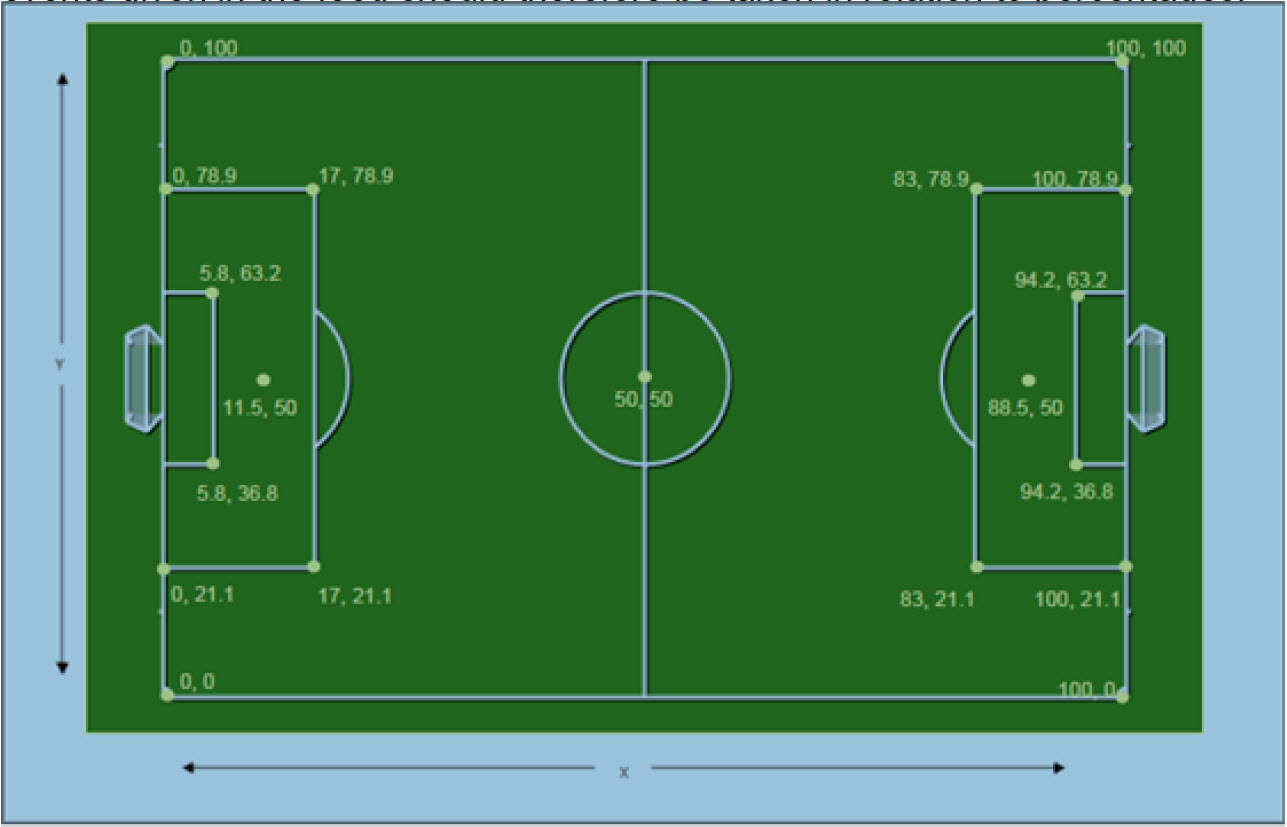
\includegraphics[scale=0.28]{se-wa-jpg/opta_pitch}
\caption[Koordinatensystem Opta]{Koordinatensystem Opta\protect\footnotemark}
\label{opta_pitch}
\end{figure}
\footnotetext{Abbildung in Anlehnung an \textit{Opta-Sports}, F24 Appendices, 2017b, S. 43.}
\enlargethispage{2\baselineskip} 
Die vorliegende Arbeit beschäftigt sich mit der Wahrscheinlichkeit eines Torerfolges von einer bestimmten Position aus. Folglich liegt der Fokus auf der Selektion aller Schüsse, die über die Type-IDs \textsf{13, 14, 15} und \textsf{16} identifiziert werden können. \vref{tab:events} gibt dazu einen Überblick über die einzelnen Events mit kurzen Beschreibungen. Aus der Tabelle können die Schüsse in die für die Funktionsmodellierung wichtigen Kategorien \textbf{Tor} und \textbf{Nicht-Tor} eingeteilt werden. Schüsse mit der Type-ID \textsf{13, 14, 15} werden demzufolge als Nicht-Tor sowie die Type-ID \textsf{16} als Tor verbucht.

%%%%%%%%%%%%%%%%%% Tabelle Schüsse %%%%%%%%%%%%%%%%%%
\tablefirsthead{\hline\multicolumn{3}{|c|}{\textbf{Schuss-Events}}\\\hline\hline \textbf{Type-ID} & \textbf{Name} & \textbf{Beschreibung}\\\hline}
\tablehead{\hline \textbf{Type-ID} & \textbf{Name} & \textbf{Beschreibung}\\}
\tabletail{\hline \multicolumn{3}{|r|}{\textsl{Fortsetzung nächste Seite}}\\\hline }
\tablelasttail{}
\bottomcaption{Schuss-Events\label{tab:events}}
\begin{center}%
\begin{supertabular}{ | P{2cm} | P{3cm} | P{5cm} |}
\vspace*{1mm} 13 	& \vspace*{1mm}Miss  	& Jeder Schuss, der am Tor vorbei ging	\\
\hline
\vspace*{1mm}14	& \vspace*{1mm}Post	& Der Ball hat den Torrahmen getroffen 	\\
\hline
\vspace*{1mm}15	& \vspace*{1mm}Attempt Saved  	& Alle Schüsse, die gehalten wurden	\\
\hline
\vspace*{1mm}16\vspace*{1mm}	& \vspace*{1mm}Goal\vspace*{1mm}  	& \vspace*{1mm}Alle Tore\vspace*{1mm}	\\
\hline
\end{supertabular}
\end{center}

Aus der dritten Anforderung (vgl. Auflistung der Anforderung \vref{tab:anf}) lässt sich schließen, dass für die Modellierung nur Schüsse berücksichtigt werden dürfen, die aus dem \glqq \textit{laufenden}\grqq~Spiel abgegeben wurden. Die Qualifier \textsf{9, 25} und \textsf{26} geben darüber Aufschluss, ob ein Schuss aus einer Standardsitutation (Eckball, Freistoß oder Elfmeter), also nicht aus dem laufenden Spieler heraus, hervorgeht. Ferner müssen Eigentore ausgeschlossen werden, da diese -- wie in Anforderung 4 beschrieben -- die Modellierung verzerren würden. Geblockte Schüsse müssen ebenfalls unberücksichtigt bleiben, anlässlich der Tatsache, dass keine konkrete Aussage getroffen werden kann, ob solch ein Schuss in einem Torerfolg resultiert hätte (vgl. Anforderung 5).\vref{tab:quali} fasst dazu nochmal alle relevanten Qualifier zusammen.

%%%%%%%%%%%%%%%%%% Tabelle Qualifier %%%%%%%%%%%%%%%%%%
\tablefirsthead{\hline\multicolumn{3}{|c|}{\textbf{Relevante Qualifier}}\\\hline\hline \textbf{Q-ID} & \textbf{Name} & \textbf{Beschreibung}\\\hline}
\tablehead{\hline \textbf{Q-ID} & \textbf{Name} & \textbf{Beschreibung}\\}
\tabletail{\hline \multicolumn{3}{|r|}{\textsl{Fortsetzung nächste Seite}}\\\hline }
\tablelasttail{}
\bottomcaption{Relevante Qualifier\label{tab:quali}}
\begin{center}%
\begin{supertabular}{ | P{2cm} | P{3cm} | P{5cm} |}
\vspace*{1mm}9 	& \vspace*{1mm}Penalty  	& 	Schussversuch resultiert aus einem Elfmeter\\
\hline
\vspace*{1mm}25	& \vspace*{1mm}From Corner  	& Schussversuch resultiert direkt aus einer Ecke 	\\
\hline
\vspace*{1mm}26	& \vspace*{1mm}Free Kick  	& Schussversuch resultiert direkt aus einem Freistoß  	\\
\hline
\vspace*{1mm}28	& \vspace*{1mm}Own Goal  	& Eigentor (inverse Koordinaten) 	\\
\hline
\vspace*{1mm}82	& \vspace*{1mm}Blocked  	& Schussversuch der geblockt wurde 	\\
\hline	
\end{supertabular}
\end{center}

Als Datenbasis für diese Arbeit wurden von Opta folgende Spieldaten aus der ersten deutschen Fußballliga bereitgestellt:

\begin{itemize}
\item Bundesliga-Saison 2013/2014 (GER)
\item Bundesliga-Saison 2014/2015 (GER)
\item Bundesliga-Saison 2015/2016 (GER)
\item Bundesliga-Saison 2016/2017 (GER)
\end{itemize}

Damit liegt eine ausreichend große und repräsentative Datenmenge mit über 15.000 verfügbaren Schüssen für eine Funktionsmodellierung vor, die im folgenden Kapitel (vgl. \vref{umsetzung}) umgesetzt wird.

